\documentclass[12pt,oneside]{report}

% \AddToHook{cmd/section/before}{\clearpage}

\usepackage[T1]{fontenc}

\usepackage{aas_macros}
\usepackage[letterpaper, top=1in]{geometry}
\usepackage{titlesec}

\titleformat{\chapter}{\normalfont\normalsize\centering}{\thechapter.}{1em}{}
\titleformat{\section}{\normalfont\normalsize\centering}{\thesection}{1em}{}
\titleformat{\subsection}{\normalfont\normalsize\centering}{\thesubsection}{1em}{}
% \titlespacing*{\chapter}{0pt}{0pt}{40pt} 
% \titlespacing*{\section}{0pt}{0pt}{20pt}
\renewcommand{\contentsname}{Table of Contents}
\AtBeginDocument{
      \renewcommand{\bibsection}{\chapter*{\bibname}}
  }

\usepackage{setspace}
\usepackage{booktabs}

\usepackage{etoolbox}% http://ctan.org/pkg/etoolbox
\makeatletter
% \patchcmd{<cmd>}{<search>}{<replace>}{<succes>}{<failure>}
\patchcmd{\@chapter}{\addtocontents{lof}{\protect\addvspace{10\p@}}}{}{}{}% LoF
\patchcmd{\@chapter}{\addtocontents{lot}{\protect\addvspace{10\p@}}}{}{}{}% LoT
\makeatother
\usepackage[tableposition=above]{caption}

\usepackage{amsmath}	% Advanced maths commands
\usepackage{txfonts}
\usepackage{hyperref}
\hypersetup{
    colorlinks=true,
    linkcolor=black,
    filecolor=black,
    urlcolor=black,
    citecolor=black,
    pdftitle={Thesis},
    pdfpagemode=FullScreen,
}
\urlstyle{same}
% \usepackage{amssymb}	% Extra maths symbols

\usepackage{graphicx}	% Including figure files
\graphicspath{{../figures/}} 
\usepackage{natbib}
\usepackage[nottoc,numbib]{tocbibind}

\usepackage{isotope}
% \usepackage[titles]{tocloft} % fig titles
% \renewcommand{\cftfigpresnum}{\figurename\enspace}
% \setlength{\cftfignumwidth}{5em}
% \renewcommand{\cfttabpresnum}{\tablename\enspace}
% \setlength{\cfttabnumwidth}{5em}



% \usepackage{fancyhdr}
% \pagestyle{fancy}
% \fancyhead{}
% \fancyhead[RO,RE]{Carbon Galactic Nucleosynthesis}
\pagestyle{plain}
\counterwithout{figure}{chapter}
\counterwithout{table}{chapter}
\counterwithout{equation}{chapter}


\defcitealias{cristallo+11}{C11}
\defcitealias{cristallo+15}{C15}
\defcitealias{ventura+13}{V13}
\defcitealias{karakas10}{K10}
\defcitealias{KL16}{KL16}
\defcitealias{karakas+18}{K18}
\defcitealias{james+21}{J21}



\newcommand{\JJ}{\citetalias{james+21}}
\newcommand{\cristallo}{\citetalias{cristallo+11}+\citetalias{cristallo+15}}
\newcommand{\karakas}{\citetalias{karakas10}}
\newcommand{\kl}{\citetalias{KL16}+\citetalias{karakas+18}}
\newcommand{\ventura}{\citetalias{ventura+13}}

\newcommand{\VICE}{\texttt{VICE}}
\newcommand{\caah}{[C/Mg]-[Mg/H]}
\newcommand{\caafe}{[C/Mg]-[Mg/Fe]}

\newcommand{\zoo}{\ensuremath{Z/Z_{\sun }}}
\newcommand{\Ycc}{\ensuremath{y_{\rm C}^{\rm CC}}}
\newcommand{\Yct}{\ensuremath{y_{\rm C, 0}^{\rm tot}}}
\newcommand{\Yoc}{\ensuremath{y_{\rm Mg}^{\rm CC}}}
\newcommand{\Ycagb}{\ensuremath{y_{\rm C}^{\rm AGB}}}
\newcommand{\sun}{\ensuremath{\odot}}


\newcommand\T{\rule{0pt}{2.6ex}}       % Top strut
\newcommand\B{\rule[-1.2ex]{0pt}{0pt}} % Bottom strut
\newcommand{\possesivecite}[1]{\citeauthor{#1}'s \citeyearpar{#1}}
\newcommand{\alp}{$\alpha$}

\newcommand{\citetjack}{JRoberts et. al (2023, in preperation)}
\newcommand{\citepjack}{(Roberts et. al 2023, in preperation)}
\newcommand{\citealtjack}{Robert et. al 2023, in preperation}

\setcitestyle{aysep={}} 
\setcitestyle{notesep={; }} 



\title{Carbon Nucleosynthesis}
% The list of authors, and the short list which is used in the headers.
% If you need two or more lines of authors, add an extra line using \newauthor
\author{Daniel A. Boyea}

% These dates will be filled out by the publisher
\date{\today}

\pagenumbering{roman}

\begin{document}

%\doublespacing


\begin{titlepage}
   \begin{center}
       \vspace*{5\baselineskip}
       \textbf{The Galactic Chemical Evolution of Carbon} \\
       Implications for Stellar Nucleosynthesis\\
       \vspace*{3\baselineskip}
        Undergraduate Research Thesis\\
       \vspace*{3\baselineskip}
    Presented in partial fulfillment of the requirements for graduation \textit{with research distinction in Astronomy and Astrophysics} in the College of Arts and Sciences of The Ohio State University \\
       \vspace*{3\baselineskip}
        by \\
       \vspace*{3\baselineskip}
       {Daniel Alexander Boyea}\\
       \vspace*{3\baselineskip}
       The Ohio State University\\
       April 2023\\
       \vspace*{3\baselineskip}
       Project Advisor: David Weinberg, Department of Astronomy
       % Rolando Vald\'es Aguilar\\
       \vfill
   \end{center}
\end{titlepage}



% Abstract of the paper
\chapter*{Abstract}
\addcontentsline{toc}{chapter}{Abstract}
Stellar evolution models provide highly uncertain predictions for elemental yields due to our limited understanding of stellar physics. In this paper, I aim to estimate the nucleosynthetic yields of C using galactic chemical evolution models. 

I find that the AGB stars make up a fraction $0.20_{-20}^{+80}$ of total C production at late times. 

\chapter*{Acknowledgements}
\addcontentsline{toc}{chapter}{Acknowledgements}

James Johnson, for guiding me through this project and through my last year of undergraduate.
Wayne Schlingman, for everything you do for everyone. You are the glue holding together our department.
David Weinberg and Jennifer Johnson, for listening to my earlier drafts of this work and providing excellent suggestions.

I also would not have made it here without all the additional support from my friends and family. Eric, even across the country, you have always been a point of support and stability, and I am always happy to be around you. Anya, you are a wonderful friend and I cannot thank you enough for your support this year. 
I love so many people in our department who have just been friends and positive support: Kaia, Maria, Autumn, Simon, Mary, Aaliyah, Sanskruti, Alyssa, Harrison, Denis, and so many others. 
My Family (and Arya, our lovely doodle).

%% Lists

\tableofcontents
\listoffigures
\listoftables
\newpage
\pagenumbering{arabic}

%%%%%%%%%%%%%%%%%%%%%%%%%%%%%%%%%%%%%%%%%%%%%%%%%%

%%%%%%%%%%%%%%%%% BODY OF PAPER %%%%%%%%%%%%%%%%%%

\chapter{Introduction}

Galactic chemical evolution (GCE) aims to understand the chemical and star formation histories of galaxies. At the core of GCE models are stellar yields---the amount of each chemical element stars produce (or destroy). The chemical elements are produced in different amounts by different stars, leaving traces of Galaxy's evolutionary history. Through \textit{Galactic Archeology}, we can reconstruct the history of our galaxy by investigating the clues left in reminants of the past \citep{Weinberg+22, emily+19}.

Here, I aim to understand C enrichment---where it is produced and how its abundances evolve over time. Why study C? C is unique nucleosynthetically, one of few light elements (along with N) produced in asymptotic giant branch (AGB) stars \citep[e.g.][]{jennifer19, KL14}. C and N are well studied elements since they are easy to observe in stellar spectra, even at the lowest metallicities \cite[e.g.][]{fabbian+09, nissen+14, lambert81, laird85, lambert86}. Additionally, C and N are used as age indicators in red giant branch stars \citep{martig16, MG15, hasselquist19, fiorenzo+21}.

Gas-phase [C/O] ratios---observed in very low metallicity, high redshift damped Lyman-alpha systems (DLAs)---decrease with increasing [O/H] \citep{FN15, cooke+17}. Then, [C/O] increases above $\rm [O/H] \approx 1$ (\citealt{berg+19}; see discussion in \S\ref{sec:gas}).
While we know C is produced in AGB stars and core collapse supernovae (CCSNe), we still have limited understanding of the magnitude and metallicity-dependence of each process.


Despite their central role in GCE models, nucleosynthetic yields predicted by stellar evolution models are rife with uncertainties. The production rates of elements in stars are shaped by poorly understood processes, including mass loss, opacity, nuclear reaction rates, rotational mixing, and convection\citep{KL14,ventura+13, LC18}.
Additionally, changes in massive stars' explodability introduce further variation in population averaged-yields \citep{emily+21}.

GCE models typically use unmodified nucleosythetic predictions and attempt to create models matching observations by varying the star formation history (SFH) and other evolutionary parameters. I choose to introduce C yields as a free parameter, determining which yield prescriptions reproduce Galactic abundance trends.
\cite{james+22} examined similar GCE models of N, an element whose production is closely related to C. \cite{james+22} found trends in N and O abundances can be explained by the metallicity dependence of relative N and O yields. Here, I extend their models to C and show that similar constraints on C and O relative yields can be obtained from observed abundance ratios. Additionally, I assess which yield prescriptions reproduce Galactic abundance trends, while assessing the impact of SFH and GCE model assumptions.

Accurate determination of stellar birth abundances for C and N is challenging. When a star enters the red giant branch (RGB), material from the CNO-processed core is mixed with the envelope in first dredge up (FDU), enhancing N and depleting C \citep{iben67, fiorenzo+21,KL14}. Measurements of these evolved stars'  atmospheres will no longer reflect birth abundances.  Additionally, gas-phase measurments of C are extremely limited as C lacks strong lines in HII regions \citep{skillman+20}.

To this end, I use a sample of subgiant stars from APOGEE \citep{apogee17}. According to stellar evolution models (CITES), these stars have not yet experienced FDU. Their phosphoric abundances should thus represent their birth composition.  In Fig. \ref{fig:subgiants}, I plot this sample, selected by criteria in (see Appendix \ref{sec:jack}; \citealtjack). These emperical resolults contain information on the relative C and Mg yields, which I use later in this work.


\begin{figure}[htp]
    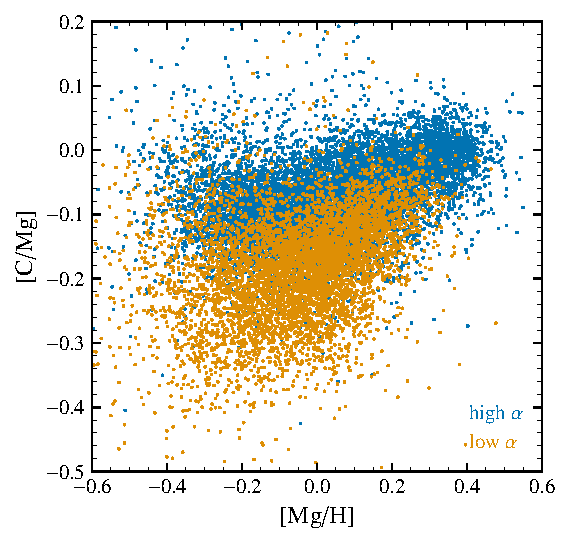
\includegraphics{subgiants_mgh.pdf}
    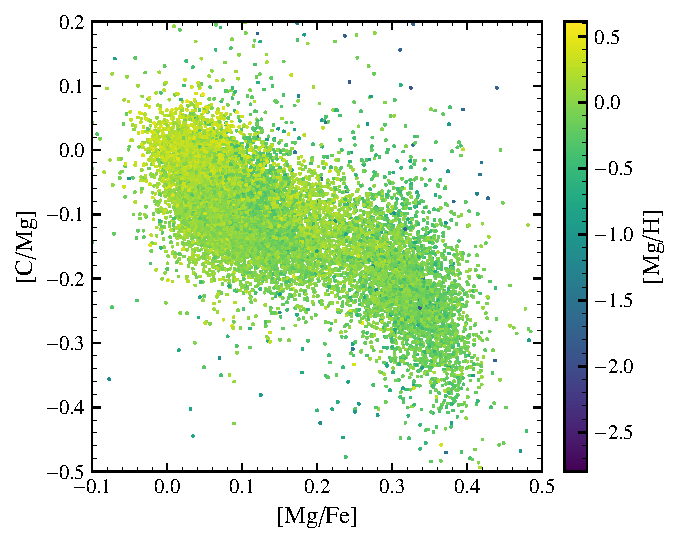
\includegraphics{subgiants_mgfe.pdf}
    \caption[APOGEE Subgiants]{The [C/Mg] ratio against [Mg/H] (top) and [Mg/Fe] (bottom) for the \citetjack~sample of APOGEE subgiants. On the top, I plot high-$\alpha$ stars in blue and low-$\alpha$ stars in orange using the seperation defined in Equation \ref{eq:high_alpha}. On the bottom, I colorcode stars according to their [Mg/H] abundance.}
    \label{fig:subgiants}
\end{figure}
\chapter{Nucleosynthesis}

Theoretical models of stellar nucleosynthesis provide the starting point of this investigation. I focus on three primary nucleosynthetic pathways: Asymptotic giant branch (AGB) stars, core collapse supernovae (CCSNe), and type Ia supernovae (SNe Ia). Each process has unique timescales and yields, traceable through the tools of GCE. While C is only produced in AGB stars and CCSNe, comparing C to Fe, which is produced in SNe Ia, adds a valuable constraint on the delay-time distribution (DTD) of C enrichment.

When a single stellar population (SSP) forms, CCSNe are the first enrichment events. CCSNe provide light elements such as C, O, and Mg and heavier elements such as Fe and beyond. Metallicity-independent yields from CCSNe are the only statistically significant source of O and Mg ($\alpha$ elements). Next, low mass stars begin to reach the end of their lives. The dying breaths of AGB stars are known to be important sources of C, N, and neutron capture elements.  Finally, white dwarfs explode, releasing Fe and other iron-peak elements.


For an element X and star with mass $M$, the stellar yield $\tilde{y}$ is defined as the net production of X relative to $M$, or
\begin{equation}
    \tilde{y}_{\rm X} = \frac{M_{\rm X,\ ejected} - Z_{0, X} M_{\rm ejected}}{M}   
\end{equation}
where $M_{\rm ejected}$ and $M_{\rm X, ejected}$  are the total ejected mass of the envelope and the element X, respectively. 

Though per-star yields are necessary to compute AGB star enrichment rates in GCE models, IMF-averaged\footnote{IMF: Initial Mass Function} yields are useful in interpreting their predictions. For a yield $y$ from a star of mass M and initial metallicity $Z$, the IMF-averaged yield is given by 
\begin{equation} \label{eq:imf-yield}
    y_{\rm X}^{\rm proc}(Z) = 
    \int_{M_{\rm min}}^{M_{\rm max}} 
    \tilde{y}_{\rm X}^{\rm proc}(M, Z)
    \frac{dN}{dM}  \ dM
\end{equation}
where ${dN}/{dM}$ is the normalized IMF, $M_{\rm min}$ and $M_{\rm max}$ are the minimum and maximum mass of stars, which I take to be $0.08 M_{\sun}$ and $100 M_{\sun}$ respectively. For AGB stars, the yields are truncated above 8 $M_{\odot}$. 
To calculate the IMF-weighted net yields of C, I use the Versatile Integrator for Chemical Evolution code (\VICE\footnote{\VICE~is available at \url{https://github.com/giganano/VICE}}).

In the interest of focusing on carbon yields, I hold yields of other elements fixed. 
I adopt yields from \citet{james+21, james+22}.
In Table \ref{tab:fiducial_mod}, I tabulate yield values, in units of a stellar population's birth mass.
Also following \citet{james+21, james+22}, I take the SNeIa delay time distribution to be a
$t^{-1.1}$ law suggested by the observations of \citet{maoz+12}.


\begin{table}
	\centering
    \caption[Fiducial Model]{Yields for the fiducial model}
	\label{tab:fiducial_mod}

	\begin{tabular}{l l l l}
		\toprule
        Element & $\Ycc$ & $\tilde{y}^{\rm AGB}$ & $y^{\rm SNe Ia}$ \\
		\midrule
        C & $0.0028 + 0.001(Z/Z_\odot)$ & $2.9\times{\rm C11}$ &  0 \\
        Mg & 0.00185 & 0 & 0 \\
        Fe & 0.0012 & 0 & 0.00214 \\
        N & 0.00072 & $9\times10^{-4}(Z/Z_\odot)M$ & 0\\
		\bottomrule
	\end{tabular}
\end{table}

\section{Asymptotic giant branch stars}\label{sec:agb}


An AGB star is a low mass ($\lesssim 8 M_{\sun}$) star during its final phase of evolution.  In an AGB star, two competing processes determine the outcome of C production: third dredge up (TDU) and hot bottom burning (HBB).  TDU accompanies thermal pulsations in AGB stars. During a TDU event, material from the CO core is mixed with material exposed to partial He-shell burning, increasing C and O abundances in the envelope \citep{KL14}.
HBB is the activation of proton capture reactions, and the CNO cycle%
\footnote{The CNO (I) cycle is
\isotope[12]{C}(p, $\gamma$)
\isotope[13]{N}($\beta^+ \nu_e$)
\isotope[13]{C}(p, $\gamma$)
\isotope[14]{N}(p, $\gamma$)
\isotope[15]{O}($\beta^{+}\nu_e$)
\isotope[15]{N}(p, \alp)
\isotope[12]{C}.
 Other minor branches of the CNO cycle are not relevant here.
 \citep{solar-fusion}.
}
at the base of the convective envelope. Because the $^{14}$N(p, $\alpha$) proton capture is the slowest component of the CNO cycle \citep{solar-fusion}, the CNO cycle converts nearly all \isotope[12]{C} into \isotope[14]{N}.
As a result, when both TDU and HBB occur, \isotope[12]{C} yields are lowered (see discussion in \citealt{james+22} and \citealt{ventura+13}).

In this work, I explore four different sets of AGB star yield tables from literature, providing well sampled grids in metallicity and mass for use in chemical evolution models. 
\begin{itemize}
    \item C11: \citet{cristallo+11, cristallo+15}
    \item K10: \citet{karakas10}
    \item V13: \citet{ventura+13,ventura+14,ventura+18}
    \item K16: \citet{KL16} \citet{karakas+18}
\end{itemize}
I use C11 as the fiducial AGB yield.


Fig. \ref{fig:y_agb} compares the AGB C yield $\tilde{y}_\text{C}^\text{AGB}(M, Z)$ for each model I consider. 
The yields may be negative when the birth abundance is higher than the C abundance of the material ejected back to the interstellar medium (ISM). 
Most models agree on the qualitative shape of the net fractional AGB C yield---% 
stars with mass $\sim 2--4 M_\odot$ have highest fractional C yields, with the mass of the peak increasing and overal yields decreasing with increasing $Z$.  High mass, high $Z$ stars destroy \isotope[12]{C} due to HBB.

In Fig. \ref{fig:agb-ssp}, we plot the total production of C by AGB stars as a function of SSP age.
Effectively, this is equivalent to integrating Eq. \ref{eq:imf-yield} down to $M_{to}$, the turnoff mass for time $t$%
\footnote{In our model, the mass-lifetime relation is
$\log \tau_M = 1.02 - 3.57\log M + 0.90 \left(\log M\right)^2$,
where $\tau_M$ is in Gyr,
from \citet{larson74}.}.
As the mass range $2\lesssim M \lesssim 4$ is most important for C production, the characteristic delay time is $\sim 1$Gyr. In contrast, Fe from SNeIa (plotted as the dashed black line in Fig \ref{fig:agb-ssp}) has a longer characteristic delay time.

K10 and K16 weight C production more heavily towards massive stars resulting in a faster enrichment delay time, whereas the C11 and V13 models predict a slightly longer timescale with order 1 Gyr, but little to no C is produced more than 2 Gyr after a star formation event. This is in contrast to iron which is still produced by SNeIa up to 10 Gyr after a star formation event. 
As shown in the right panel of Fig. \ref{fig:agb-ssp}, with increasing $Z$, C enrichment occurs earlier, and C destruction in low mass stars leads to a declining C abundance at late times.
    

\begin{figure}
    \centering
 	    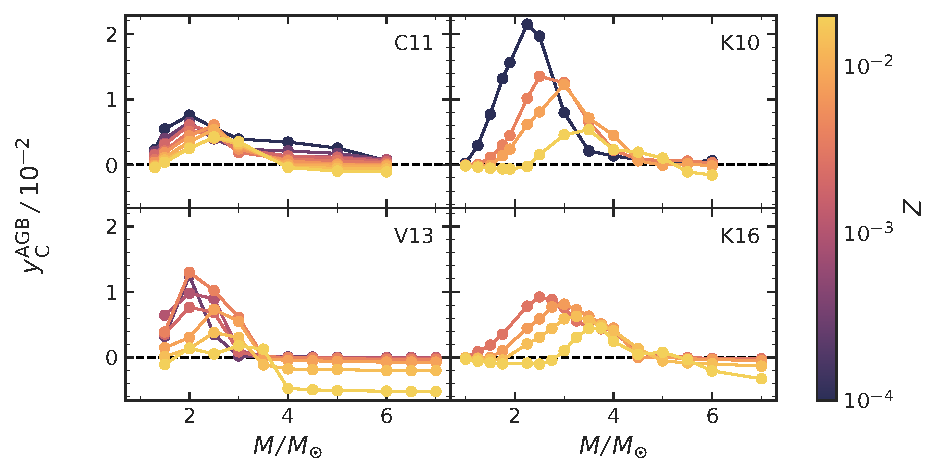
\includegraphics[scale=1]{agb_yields.pdf}
        \caption[AGB C yields]{The net fractional AGB C yield ($\tilde{y}$) plotted as a function of initial stellar mass $M$. Metallicity is colorcoded according to the colorbar. I plot $\tilde{y}=0$ for reference. Each panel represents yields from one of four AGB models: C11, K10, V13, K16 (see \S \ref{sec:agb}). }
        \label{fig:y_agb}
\end{figure}
\begin{figure}
    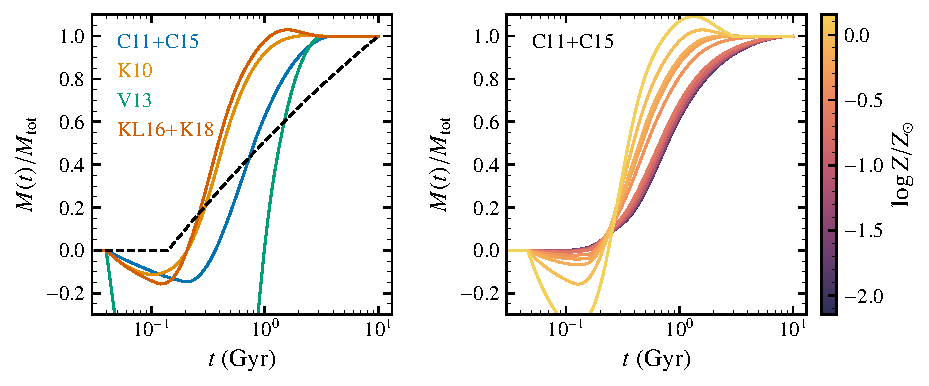
\includegraphics[scale=1]{y_agb_t2.pdf}

    \caption[AGB yields delay time distribution]{
        C production by AGB stars as a function of SSP age, normalized to the total mass $M_{\rm tot}$ produced at $t=10$ Gyr. Left: The four AGB yield models from literature at solar metallicity (C11, K10, V13, or K16). The delay time distribution of type Ia supernovae ($\propto t^{-1.1}$) is plotted as a dashed black line for comparison. Right: The C11 AGB model at different metallicities. }
    \label{fig:agb-ssp}
\end{figure}


In Fig. \ref{fig:yagb-z}, I plot the IMF-averaged C yields for each AGB model as a function of metallicity $Z$.
V13 differs that it shows a non-monotonic metallicity dependence. However, this effect is only form models with $\log Z/Z_\odot \lesssim -1$.
Otherwise, models only differ in the yield normalization and strength of metallicity dependence. All models predict yields within a factor of $\sim 2$.
For example, the three models C11, K10, and K16 predict $y_\text{C}^\text{AGB}$ to be between 0.006 and 0.008 at solar metallicity, but C11 has a much shallower metallicity dependence than the K10 and K16 models. V13 instead predicts a yield $\sim 0.004$.

\begin{figure}
    \centering
    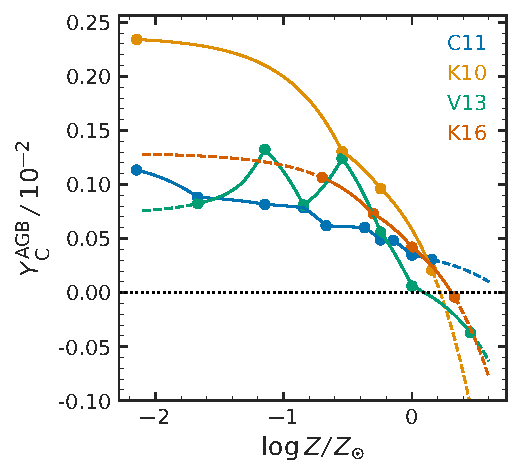
\includegraphics[scale=1]{y_agb_vs_z.pdf}

    \caption[AGB yield metallicity dependence]{The net fractional IMF-weighted AGB C yield $\Ycagb$ as a function of metallicity for each of our AGB yield models.
    }
    \label{fig:yagb-z}
\end{figure}

\section{Core collapse supernovae}


Massive stars form $^{12}$C in their cores through the triple--$\alpha$ process. However, only C ejected through supernovae and stellar winds contributes to the yield. 
While there are many stellar models providing predictions of CCSNe yields, the results of these models are highly uncertain due to the many stellar modeling uncertainties. 

In Fig. \ref{fig:y_cc}, I plot calculations of the IMF-integrated yields, using Eq. \ref{eq:imf-yield} (computed using \VICE's \texttt{vice.yields.ccsne.fractional} function). 
CCSNe models predict a wide range of C yields, spanning almost 1 dex. 
Both the \citet{NKT13} and \cite{LC18} models show positive metallicity dependence. 
The \cite{LC18} models also include rotation, showing that variations in the rotational velocity of the star can dramatically increase C production and the metallicity dependence of $\Ycc$. Rotation induces more mixing allowing the CO core to grow larger. Our fiducial model's steep metallicity dependence near $Z\approx Z_\odot$ could be explained by rotation. 


I show the C11 model for comparison in Fig. \ref{fig:y_cc}. Especially at $Z\approx Z_\odot$, most CCSNe models would dominate C production. I will later show that empirically, CCSNe also dominate C production. 

On the bottom of Fig. \ref{fig:y_cc}, I also show the CCSNe-[C/Mg] ratio, defined by
\begin{equation}\label{eq:c_mg_cc}
    {\rm [C/Mg]^{CC}} = \log_{10}\left( \frac{\Ycc}{\Yoc}\right) - \log_{10} \left( \frac{Z_{{\rm C},\ \sun }}{Z_{{\rm Mg},\ \sun }} \right).
\end{equation}
In other words, ${\rm [C/Mg]^{CC}}$ describes what [C/Mg] would be if CCSNe were the only process producing C.
Once again, different CCSNe models span a large range in [C/Mg]. 
I chose to instead parameterize $\Ycc$ to enable agreement with observations, as most CCSNe models fail to achieve near-solar [C/Mg].

Assumptions about the explodability landscape affect C and Mg production. Increasing the fraction of stars which explode increases $\Ycc$, as stars which directly collapse do not contribute to explosive yields \citep{emily+21}. However, C is relatively unaffected by the black-hole landscape, as very massive stars contribute carbon through enriched winds. Since Mg is formed deeper in the core of massive stars, the Mg yield drops much more steeply, so models where few stars explode (S16/W18) result in much higher [C/Mg].

CCSNe models also struggle to reach solar [O/Mg], either due to overproduction of O or underproduction of Mg \citep{emily+21}. Here, I assume ${\rm [O/Mg]} = 1$, which is not compatible with CCSNe models but is consistent with observations \cite{Weinberg+19, Weinberg+22}.
    

\begin{figure}[htp]
    \centering
    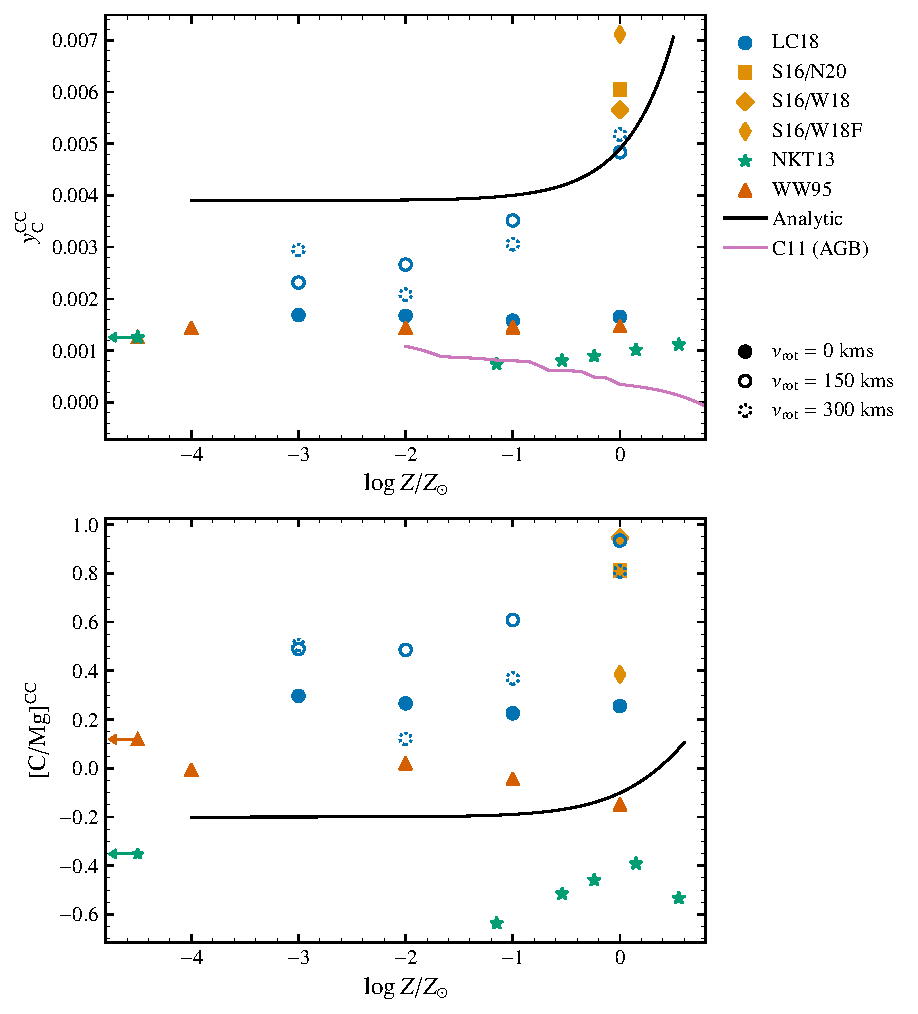
\includegraphics{y_c_cc.pdf}
    \caption[CCSNe C yields]{
        C yields from massive stars.
        Top: The IMF-weighted CCSNe yield of C a function of metallicity.
        Bottom: The CCSNe [C/Mg] abundance ratio, defined in Eq. \ref{eq:c_mg_cc}. The black line represents the C yield of the fiducial model,
    $\Ycc = 0.0028 + 0.001 (Z/Z_{\odot})$. 
    \citet[red triangles]{WW95}, \citet[orange squares and diamonds]{sukhbold+16}, 
    \citet[green stars]{NKT13}, and \citet[blue circles]{LC18}. \citet{sukhbold+16} report yields for different black hole landscales, while \citet{LC18} provide yields at different roational velocities.
The pink line represents the C11 AGB model.
}
    \label{fig:y_cc}
\end{figure}

\chapter{The Equilibrium Approximation}\label{sec:equilibrium}

In the presence of metal-poor gas accretion and feedback-driven outflows, galaxies reach an equilibrium abundance in which production of new metals is balanced by losses to new stars and outflows \citep{larson72, dalcanton07, FD08, PS11, lilly13}.
While our galaxy is likely not in perfect equilibrium or described by a single, homogenous chemical region, the equilibrium approximation is nevertheless useful in understanding yields and metallicity dependence \citep[e.g.][]{james_dwarf,james+22,WAF17}. 

I assume a simple ``one-zone'' chemical evolution model \cite[e.g.][]{tinsley80, pagel09, matteucci21}.  The gas and stars are homogenously and instantaneusly mixed, so spacial dependence is neglected.

I define $M_{X}$ to be the mass of element X in the gas phase, $\dot{M}_\star$ to be the star fomation rate (in M$_\odot$ yr$^{-1}$), and $\eta$ to be the mass loading factor $\eta\equiv\dot{M}_{\rm outflow}/\dot{M}_\star$ representing the strength of outflows. 
SSPs return a fraction $r$ of their birth mass back to the ISM, due to ejected stellar envelopes. $r\approx0.4$ for a \citet{kroupa01} IMF.
Given the IMF-weighted yield of Mg $y_{\rm Mg}$, the rate of change in the ISM mass of Mg $\dot{M}_{\rm Mg}$ is a simple sum of sources and sinks,
\begin{equation}
    \dot{M}_{\rm Mg} = \dot{M}_{\rm Mg,~new} - \dot{M}_{\rm Mg~remnants} - \dot{M}_{\rm Mg,~outflows},
\end{equation}
where the first term on the right-hand side describes CCSNe enrichment. 
In terms of the return mass fraction of stars $r$, the mass lost to remnants is $Z_X (1-r)\dot{M}_\star$.  And, the outflows deplete a mass $Z_X \eta\dot{M}_\star$. Substituting om fpr $\eta$ and $r$,  
\begin{equation}
    \dot{M}_{\rm Mg}= y_{X} \dot{M}_\star - (1 + \eta - r) Z_{X} \dot{M}_\star.
\end{equation}
Assuming an exponentially declining star formation history $\dot{M}_\star \propto e^{-t/\tau_{\rm sfh}}$, the equilivrium abundance is derived analytically by setting $\dot{Z}_{Mg}=0$.
\begin{equation}\label{eq:z_eq}
    Z_{\rm Mg}^{\rm eq}(R) = \frac{y_{\rm Mg}}{1 + \eta(R) - r - \tau_\star / \tau_{sfh}}
\end{equation}
In the special case of constant star formation, $\tau_{\rm sfh}\to\infty$, simplifying the denominator to $1+\eta-r$.

While Equation \ref{eq:z_eq} can be applied to CCSNe C, the delayed nature of AGB C can complicates thes expression. Instead, using a DTD-integrated yield, $\langle \Ycagb \rangle$ enrichment is
\begin{equation}
    \langle \Ycagb\rangle = \frac{\int_0^T \tilde{y}_{\rm C}^{\rm agb}(M, Z) \dot{M}_\star(T - t) \frac{dN}{dM} \frac{dM}{dt} dt  }{ \dot{M}_\star \int_0^T \frac{dN}{dM} \frac{dM}{dt} dt}
\end{equation}
Eq. \ref{eq:z_eq} becomes
\begin{equation}
    Z_{\rm C}^{\rm eq}(R) = \frac{\Ycc + \langle\Ycagb\rangle}{1 + \eta(R) - r - \tau_\star / \tau_{sfh}}
\end{equation}
Taking the ratio of $Z_{\rm C}$ and $Z_{\rm Mg}$, 
\begin{equation}\label{eq:z_co}
    \frac{Z_{\rm C}^{\rm eq}}{Z_{\rm Mg}^{\rm eq}} = \frac{\Ycc + \langle \Ycagb \rangle }{\Yoc}.
\end{equation}

Analogous to \cite{james+22} arguments about N, the trends in abundance ratios are set by yield ratios in these GCE models. The effect of other GCE parameters (most importaintly $\eta$) cancels. As a consequence, yield ratios should establish abundance ratio trends in models which assume a different normalization of element yields and mass-loading (see discussion below).
This argument can also be inverted to infer  yields from abundance ratio trends. To the extent that observed C and Mg trends reflect the equilibrium abundances in different Galatic regions, we can infer the CCSNe yield given an assumed AGB star yield (or vice versa). Inffering $\Ycc$ from $\Ycagb$, 
\begin{equation}
    y_\text{C}^\text{CC} =  y_\text{Mg}^\text{CC} \frac{Z_\text{C,~eq}}{Z_\text{Mg,~eq}} - \langle y_c^{agb} \rangle
\end{equation}
Rewriting this expression as a relative yield of C and Mg,
\begin{equation}
    \frac{\Ycc}{\Yoc} = \frac{Z_{\text{C},~\odot}}{Z_{\text{Mg},~\odot}} 10^{\rm [C/Mg]} - \frac{\langle \Ycagb \rangle}{\Yoc}.
\end{equation}

\section{Yield Models}

If $\Ycc$ gets us to ${\rm [C/Mg] } \approx -1$, then $\Yct = 0.005$, but if 0, $y\approx0.006$. 
Section 2.2, additional AGB yield 1part per thousand?, Motivate AGB yield ...

Outflow yield degeneracy.
One challenge of chemical evolution models is that outflows and yields are degenerate. To avoid this degeneracy, I instead constrain relative yields. As Equation \ref{eq:z_co} shows, the yield ratios are independent of $\eta$, and independent of the SFH (ignoring the DTD term).
As such, I set the total C yields to 
\begin{equation}
    \Yct = \Ycc + \Ycagb = 0.005 \frac{\Yoc}{0.00185}
\end{equation}

is reasonably consistant with the value in \citet{asplund+09} of $Z_{\rm
C}/Z_{\rm O}=0.413$ and was chosen as to match the median value of our sample
at $Z=Z_{\sun }$. 

Additionally, each AGB yield set (C11, K10, V13, K16), fails to produce enough AGB C for our fiducial model (see REF). So, I introduce a process factor, $\alpha_{\rm AGB}$, which represents the multiplicative increase in $\Ycagb$ from the published yields.
\begin{subequations}
    \begin{align}
        \Ycagb &\rightarrow \alpha_{\rm agb}  \Ycagb \\
        \alpha_{\rm agb} &= f_{\rm agb} \frac{\Yct}{\Ycagb} \\
        \alpha_{\rm CC} &= (1 - f_{\rm agb}) \frac{\Yct}{\Ycc}.
    \end{align}
\end{subequations}

I have investigated uniform increases in C yields and have found these changes make little effect on the resulting trends. Fixing the total C yield at solar reduces the number of free parameters and keeps the model reasonably consistant with observations, and enables us to more consistantly explore differen AGB models. 

Fitting this relationship to data (figure \ref{fig:analytic}).
I find that a linear dependence on metallicity,


\begin{equation}
    \frac{\Ycc}{\Yoc} = b + \zeta \frac{Z}{Z_\odot}
\end{equation}

\begin{figure}
    \centering
    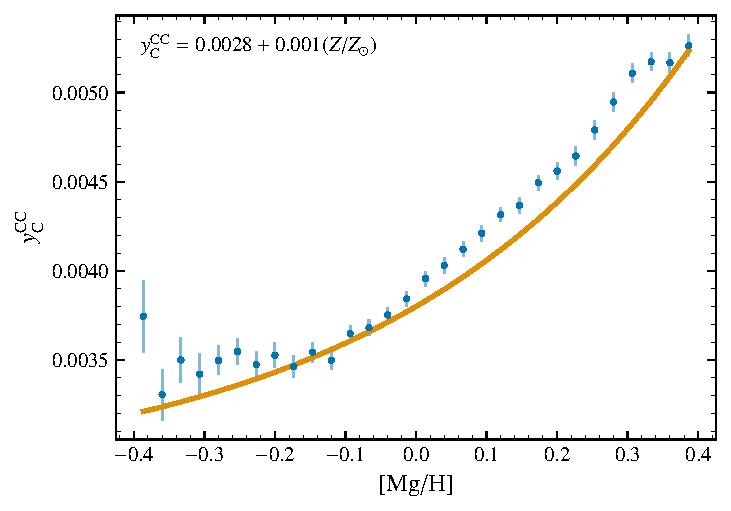
\includegraphics[]{analytic.pdf}
    \caption[Reverse fit yields]{Inferred massive star C yields as a function of metallicity. I assume equilibrium and $3\times {\rm C11}$ AGB yields (orange curve, see discussion in Section \ref{sec:equilibrium}). The binned medians and median absolute devation (divided by $\sqrt{N}$) are blue points.
    }
    \label{fig:analytic}
\end{figure}




\begin{table}
	\centering
    \caption[AGB net solar IMF yields]{For each AGB yield set, our calculation of the effective SFH- and IMF-weighted C AGB yield, along with the multiplicative factor to reach an AGB contribution of 20.}
	\label{tab:alpha_agb}
	\begin{tabular}{lcr} % four columns, alignment for each
		\toprule 
		AGB Model & $y_{\rm C, 0}^{\rm AGB}$ & $\alpha_{\rm AGB, 20}$\\
        \midrule
		C11 & 0.000347 & 2.9\\
		K10 & 0.000585 & 1.7\\
		V13 & 0.000060 & 16.5\\
		K16 & 0.000421 & 2.4\\
		\bottomrule
	\end{tabular}
\end{table}


\section{Uncertainties}

I only perform this analysis on the C11 yields because the range of metallicities of the data (about [M/H] = -0.4, 0.4) only represents about 2 AGB models, relying heavily on our choice of extrapolation. C11 have a finer model grid, allowing us to have 5 theoretical predicted points within this metallicity range, allowing us to be more certain of our conclusion. 

I do note that this analysis fails to take into account selection effects and biases in APOGEE, and a more robust determination of the C yield. 


This formulation is degenerate in $\alpha_{\rm CC}$ until I estimate a better AGB fraction. As the seperation between the low and high alpha sequences can be used to estimate the delayed time contribution to C, using the model to estimate this value relies heavaly on the details of the SFH in addition to the 
I do give an estimate of the CCSNe yields, however this is dependent on our choice of $\eta$. Other choices of $\eta$ vary the value significantly in both magnitude and slope (as AGB contributions increase, I need less CCSNe C, however the CCSNe C must have a higher metallicity dependence to replicate the V21 data). 



\chapter{The Multizone Model}\label{sec:vice}

Classical, ``one-zone'' models of chemical evolution assume instantanius mixing of metals in the star forming ISM \citep[e.g.][]{matteucci21}. This simple framework is a poor approximation for the Milky Way.  The Galaxy evolves ``inside out''---where star formation is higher towards the center and in the early universe \citep{bird+13}. Additionally, stars can migrate several kpc over their lifetimes, mixing together different chemical environments across the galaxy \citep{bird+12,sellwood+binney02}. For the rest of this paper, I focus on multizone models, which discretize the Galaxy into concentric annuli and allow stare to move between rings.  Specifically, I make use of the \citet{james+21} (hereaafter \JJ) model for the Milky Way, which runs using the publicaly available Versatile Integrator for Chemical Evolution (\VICE). This model is described extensively in \JJ~and consicely summarized  in \citet{james+22}. Here, I provide a prief overiview of the relevant model components.

In the model, the Galaxy is divided into 200 rings, each 100 pc wide. Each ring has a seperate stellar population and gas supply. Star formation ends beyond a radius $R=15.5$ kpc. I initially assume an ``inside-out'' Star Formation History (SFH), where the star formation surface density $\Sigma_\star$ is given by 
\begin{equation}
    \dot{\Sigma}_\star \propto \left(1-e^{-t/\tau_{\rm rise}}\right) e^{-t/\tau_{\rm sfh}}.
\end{equation}
$\tau_\text{rise}=2$ Gyr describes when the star formation rate reaches a maximum, and $\tau_{\rm sfh}$ describes the decay timescale of star formation as a function of radius $R$. \JJ~derives $\tau_{\rm sfh}(R)$ through analysis of four integral field spectroscopy surveys in \cite{sanches20}. The star formation history is normalized such that the total stellar mass reaches $M_\star=5.17\times10^{10} {\rm M}_\odot$ \citep{LM15} and at each $R$ to match the stellar surface density gradient \citep{BHG16}.
The gas inflow is calculated to maintain our chosen SFR for each radius and time. The gas-SFR law is based on an extension of a Kennicutt-Schmidt law \citep{kennicutt98}, motivated by 
\begin{equation}
\dot{\Sigma}_{\star} \propto \\
\begin{cases}
    {\Sigma}_{\rm gas} & 2\times 10^7 \leq \Sigma_{\rm gas} \\ 
    {(\Sigma}_{\rm gas})^{3.6} & 5\times 10^6 \leq \Sigma_{\rm gas} < 2\times10^7 \\ 
    {(\Sigma}_{\rm gas})^{1.7} & \Sigma_{\rm gas} < 5\times10^6 \\ 
\end{cases}
\end{equation}
The scaling of this relationship varies with time due to the redshift dependence of $\tau_\star$ in molecular gas observed by \citet{tacconi18}. I assume a Kroupa IMF \cite{kroupa01}.


\JJ\ accounts for radial migration by using the results of the \texttt{h277} hydrodynamical simulation \citep{christensen12, zolotov12, loebman12, BZ14}, with simulation parameters described in \citet{bird+21}. Each \VICE single stellar population (SSP) is matched to an \textit{analogue} in \texttt{H277}, chosen to form at a similar time and radius $R$. By taking the change in radius $\Delta R$ of the analogues, the SSP move to their final radii with a $\sqrt{\text{time}}$ dependence.
This relationship between displacement and time arises when migration proceeds as a consequence of the diffusion of angular momentum \citep{frankel18, frankel20}.
I do not account for radial gas flows.
Using the results of a hydrodynamical simulation without modification limits the free parameters in the model; however, I are limitied to one dynamical history. The impact of the details of a galaxy's dynamical history on its chemical evolution is unknown, and I do not explore this question here.

As the strength of outflows controls the resulting $\alpha$ abundances, \JJ~create a metallicity gradienty by defining
\begin{equation}
\eta(R) = \frac{y_{\alpha}^{\rm CC}}{Z_{\alpha, \odot}} 10^{(-0.08\text{ kpc}^{-1})(R-4\text{ kpc})+0.3} + r - 1.
\end{equation}
This choice of $\eta(R)$ results in a [$\alpha$/H] gradient consistant with Milky Way observations \citep{james+21}. I explore models with reduced outflows in \S\ref{sec:outflows}; however, the overall scaling of yields is unknown and this model is insensitive to this normalization.


\chapter{Multizone model results}
\section{Data Selection}

\citet{james+22} compare their model against the \cite{fiorenzo+21} sample of APOGEE \citet{apogee17} red giants whose C and N abundance have been corrected for mixing process using MESA stellar evolution models. 
I instead use the \citetjack~sample of APOGEE subgiants. Subgiant stars have not undergone FDU, so their atmospheric C and N abundances are still reflective of their birth abundances and do not need mixing corrections. I additionally only compare the models to the low-$\alpha$ sequence.  The selection criteria and differences between the samples are described in Appendix \ref{sec:jack}



\section{The Evolution of C across the galaxy and through time}

Here, I present the time evolution of our fiducial model. In the next sections, I will discuss the choice of parameters and agreement with observations. Our fiducial model uses the C11 AGB yield tables (see \S\ref{sec:agb}, and Table \ref{tab:fiducial_mod}), and I amplify the C11 yields by a factor of 2.9 so that $f_{\rm AGB} = 0.2$.

The fiducial model has the following qualitative characteristics of its C yields: (a) C is predominantly produced in CCSNe, (b) CCSNe produce more C at higher metallicities, (c) AGB stars produce less carbon at higher metallicities. 

The evolution proceeds as follows.
Initially, CCSNe dominate production. As $\Ycc$ has strong metallicity dependence, [C/Mg] increases with time. Shortly thereafter, AGB stars contribute delayed C, increasing [C/Mg] even more steeply. As Mg begins to reach equilibrium, the [C/Mg] ratio plateaus as C approaches equilibrium. Finally, as $\Ycagb$ decreases or even becomes negative with higher metallicity, the [C/Mg] abundance may decline slightly. 


I show the time evolution tracks of the fiducial model in Fig. \ref{fig:c_evo} for \caah~ and \caafe~. Comparing [C/$\alpha$] against [Mg/Fe] enables us to see late time evolution of C more clearly. Because of the extended DTD of SNeIa enrichment, [Fe/H] takes longer to reach equilibrium as half of iron production comes from type-Ia supernovae, the late time evolution is not as clustered as [$\alpha$/H].

This is even more evident in the lower panel of Fig. \ref{fig:c_evo}. While the \caah~trend reaches equilibrium at $\sim5$ Gyr, the \caafe~trend continues to evolve even until the present day, exposing the effect of the relative delay times of AGB stars and SNeIa.


\begin{figure}
\centering
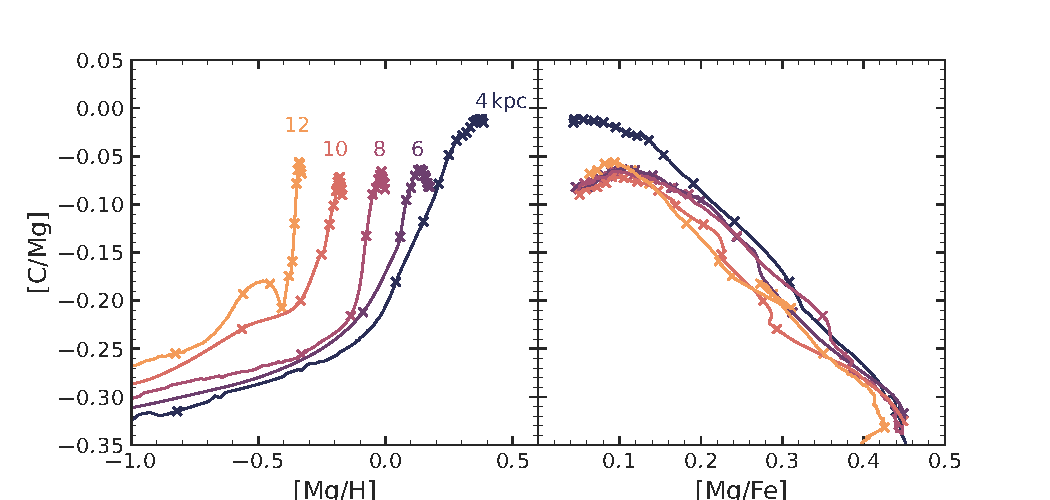
\includegraphics{evo_tracks.pdf}
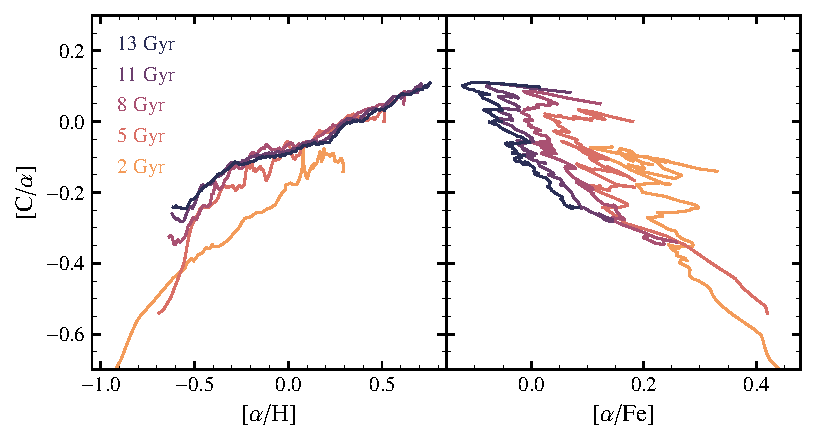
\includegraphics{evo_slices.pdf}
\caption[C chemical evolution tracks]{
    Time evolution of gas phase C abundances in our fiducial model.

    Top: Evolutionary tracks parameterized by time at fixed Galactocentric radius in the \caah and \caafe planes. 

    Bottom: snapshots of the gas-phase \caah~and \caafe~trend, parameterized by radius at fixed time.
}
\label{fig:c_evo}
\end{figure}

\section{Alternate Models}

In Fig. \ref{fig:agb_sims}, I compare the K10, K16, C11, and V13 yield models. Each model uses the published, unscaled yield tables. As the highest AGB yield at solar, K10, is only $\Ycagb=0.000585$, $f_{\rm AGB} \leq 0.12$ for all models. Massive stars dominate C production with unscaled yields.  While it is easy to modify the AGB yields in my model, their small contribution reduces the effect. I leave a more detailed discussion of the effects of AGB models for Appendix \ref{sec:alt_agb} and use C11 yields hereafter.

\begin{figure}
\centering
\includegraphics{oob_agb.pdf}
\caption[AGB GCE Models]{
    Stellar abundance trends in our model, assuming metallicity independent $\Ycc$. Colored lines quantify the median [C/Mg] in bins of [Mg/H] for our four AGB yield models from the literature (see \ref{sec:agb}). Black points and grey dashes represent the median and standard deviations in the \citetjack~sample. In the right panel, I show the trends only for stars where $-0.15\leq {\rm [Mg/H]}\leq -0.05$.
}
\label{fig:agb_sims}
\end{figure}

Next, I investigate adjustments to $f_{\rm AGB}$ and the CCSNe metallicity dependence $\zeta$ in Fig. \ref{fig:beta_f}. 

As I display in Fig. \ref{fig:beta_f}, I observe that changes in $\beta$ are
approprietly reflected in the resulting \caah~trend. As the metallicity
dependence steepens with higher $\beta$, the [C/Mg] ratio becomes
correspondingly more dependent on [Mg/H].

As disscused in \S\ref{sec:equilibrium}, the \caah~trend in these models arises as a consequence o fthe relative yield $y_{\rm C}/y_{\rm Mg}$ and its metallicity dependence. This is determined by both the AGB fraction $f_{\rm AGB}$ and the metallicity dependence of CCSNe yields $\zeta$. As a result, there is a degeneracy between the two. I can increase $f_{\rm AGB}$ and $\zeta$ correspondingly, and \caah~would remain unaffected.

This degeneracy is broken by the \caafe~relation. The relationship is set by $f_{\rm AGB}$, because a specific amount of C must be released at a delayed time in order to match the SNeIa production of Fe and increase [C/Mg] as [Mg/Fe] decreases to reproduce the data.
One source of theoretical uncertanty in this result is that the SNeIa yield and DTD have their own uncertainties. I discuss variations in $y_{\rm Fe}^{\rm Ia}$ in Appendix \ref{sec:alt_agb}, and find that the quanlitative conclusions are largely unaffected. I therefore focus on the choices of $y_{\rm Fe}^{\rm Ia} = $FILLIN choices from the fiducial model here.


Due to instantaneous CCSNe enrichment, the \caafe~relation is approximantly independent of $\zeta$. I can therefore choose $f_{\rm AGB}$ such that the \caafe~relation is reproduced, and then choose $\zeta$~to simulatneously reproduce \caah. Indeed, the positive slope of the \caah~relationship compared to our GCE models is a clear indication that metallicity dependent yields from massive stars must dominate AGB star production of C. Otherwise,  the inverse dependence of $\Ycagb$ on $Z$ makes it extremelly difficult to reproduce a positive slope in \caah. If this relationship indeed arises as a consequence of chemical equilibrium and yield ratios, then a positively sloped \caah~relation with high $f_{\rm AGB}$ should only arise if the Galaxy is significantly far from equilibrium. 

C as an equilibrium phenominon. See section \ref{sec:equilibrium} Importantly, the \caafe trend is mostly unaffected by choosing a different
CCSNe yield. As all CCSNe enrichment happens at the same, rapid timescale, by
taking a slice in [Mg/H], this metallicity dependence is effectively ignored as
the only effect can be a vertical offset if the slice is narrow enough. 

So, the scaling of the trend and metallicity dependence of C (as seen in
the \caah~trend) gives information on the total C yield and the behavior
of CCSNe (as the dominating producer of C);
the \caafe trend exposes the delayed effect of C from AGB contribution.

V21 observes a significant seperation implying a more substantial delayed-time source. 


\begin{figure}
\centering
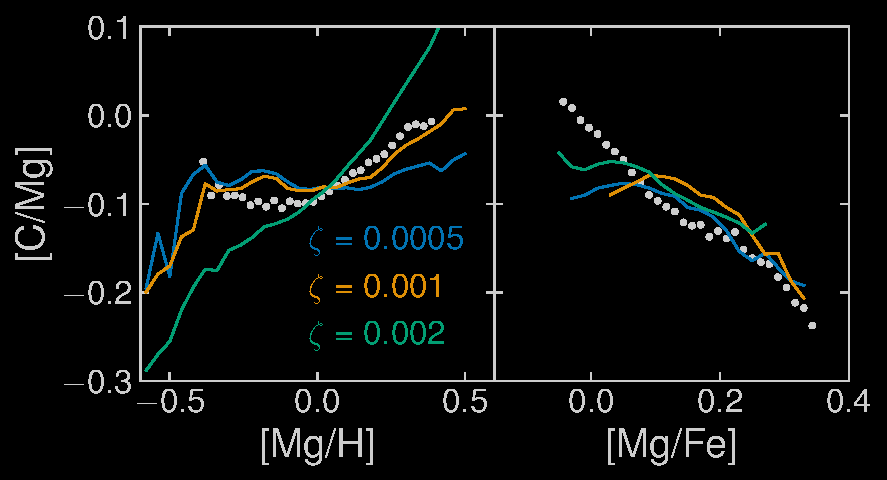
\includegraphics{beta.pdf}
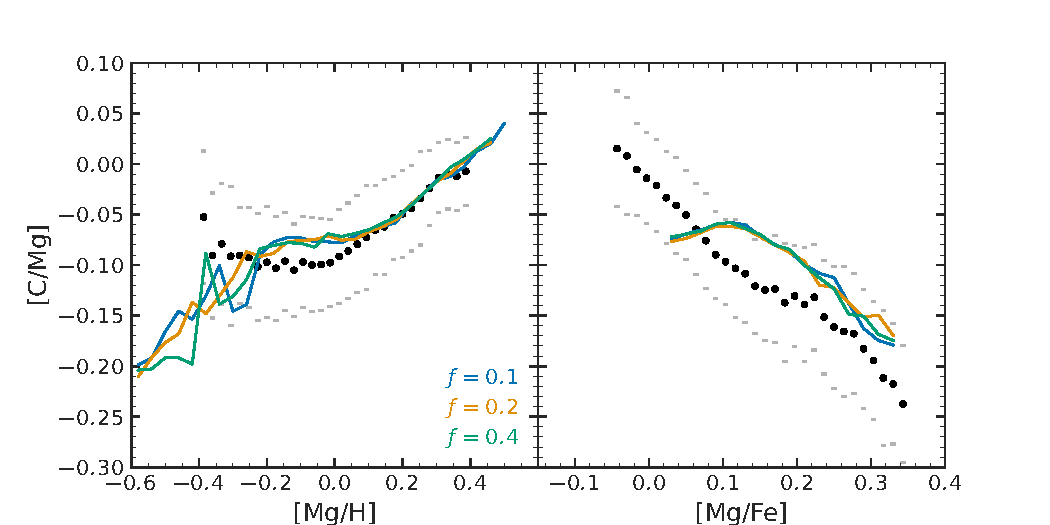
\includegraphics{f_agb.pdf}

\caption[Adjusted yield models]{Similar to Figure \ref{fig:agb_sims} except the top plot shows the fiducial model with lower and higher values of $\zeta$, the C-CCSNe metallicity dependence. The bottom plot shows models with $f_{\rm AGB}=$0.1, 0.2, and 0.4. Both the $f_{\rm AGB}$ and $\zeta$ influence \caah, but only $f_{\rm AGB}$ has a significant impact on \caafe.}
\label{fig:beta_f}
\end{figure}



\section{Star Formation History} \label{sec:sfh}



\begin{figure}
\centering
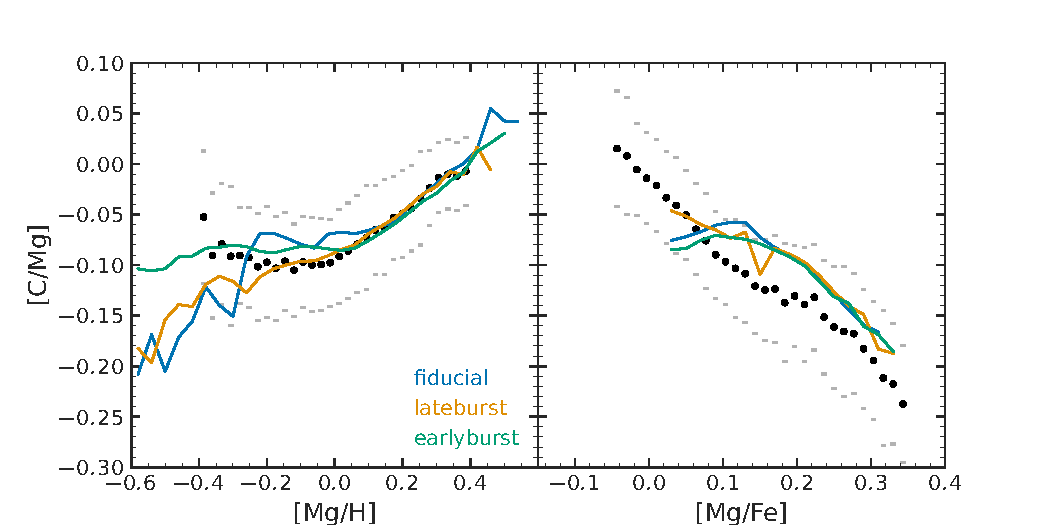
\includegraphics{lateburst_eta.pdf}

\caption[Lateburst models]{Same as Figure \ref{fig:agb_sims} but comparing the fiducial model to alternate star formation histories (see \S \ref{sec:sfh}).}
\label{fig:sfh_models}

\end{figure}


Here, I consider a "lateburst" model, created by multiplying our fiducial "inside-out" SFH with a gaussian.
\begin{equation}\label{eq:lateburst}
    \dot{\Sigma}_{\rm lateburst} \propto \dot{\Sigma}_{\rm insideout} \left(1 + A e^{-(t-\tau_{\rm burst})^2/2\sigma^2_{\rm burst}} \right)
\end{equation}

$A=1.5$ represents the amplitude of the birth, $\tau_\text{burst}=10.8$Gyr is the time where the burst is strongest, and $\sigma_\text{burst}=1$Gyr is the width of the burst.

I also consider an earlyburst model as a slight variation of the lateburst, where the burst is instead exponential and placed at $t_1=5$ Gyr. This approximantly corresponsed to the Gaia-Encelidus merger, inducing higher star formation in the Milky Way \citep{bonaca20, helmi18}.
\begin{equation}\label{eq:twoinfall}
    \dot{\Sigma}_{\rm early-burst} \propto \dot{\Sigma}_{\rm insideout} + 
\begin{cases}
    Ae^{-(t-t_1)/\tau_{\rm burst}} & t_1 < t \\
      0 & t<t_1
\end{cases}
\end{equation}
where I take the burst duration, $\tau_{\rm burst}=1$ Gyr in this case. 
This more drastic burst is able to more successfuly populate the high-$\alpha$ sequence. I leave more detailed exploration of the effects of star formation histories to future work.

I show these variations on the star formation history in figure \ref{fig:sfh_models}.


\section{Outflows} \label{sec:outflows}

GCE models of the Milky Way fall into two classes---those which incorperate significant mass-loading (e.g., as in this work) and those which neglet mass-loading but lower effective yield to match observed abundances \citep{MCM13, MCM14, spitoni19, spitoni20, spitoni21}.
An increase in stellar yields has a nearly identical effect as a decreease in the mass-loading factor $\eta$ (see Appendix B of \cite{james_dwarf}).
The equilibrium arguments discussed in \S\ref{sec:equilibrium} suggest howerver that abundance ratios are independent of the choice of normalization and the value of $\eta$. We therefore expect our results regarding the relative yield $y_{\rm C}/y_{\rm Mg}$ and its metallicity dependence to extend to the other class of models omitting mass loading. I demonstrate this further here.

The theoretical motivation for decreasing yields is the uncertainty in stellar explodability.
If fewer massive stars explode, then the yields will be reduced by some factor. Additionally, some fraction of SN ejecta may be lost directly to an outflow, lowering effective yields. To explore reduced outflow models, I lower both $\eta$ and all yields by the same factor to leave the equilibrium abundances unchanged. 

\begin{figure}

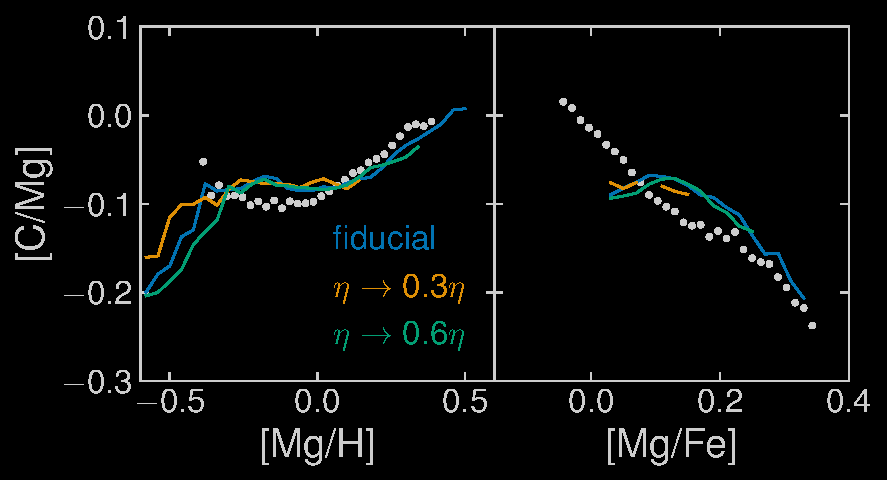
\includegraphics{eta.pdf}

\caption[Reduced-outflow models]{Same as Figure \ref{fig:agb_sims} but comparing the fiducial model to reduced outflow models (see \S \ref{sec:outflows}).}
\end{figure}


\section{Scatter}

Beyond simply comparing median trends, I can compare the distribution 

\begin{figure}
    \centering
    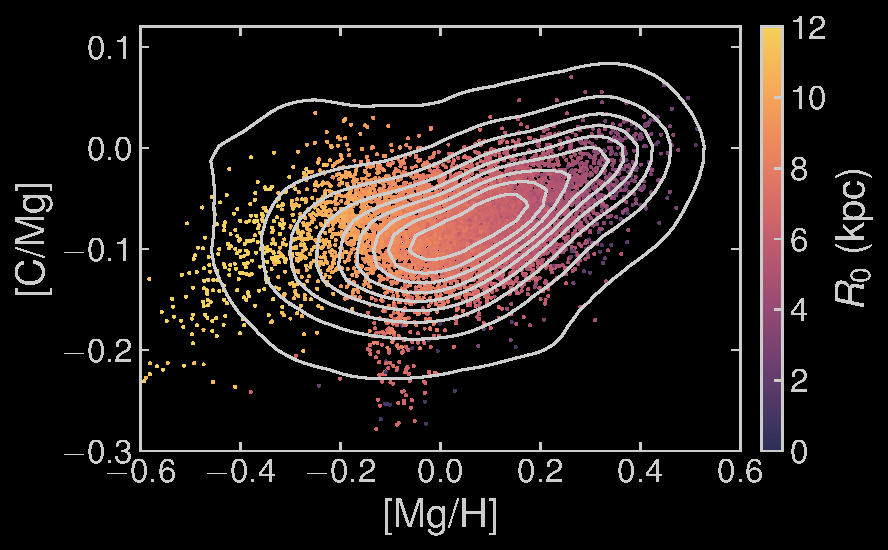
\includegraphics[scale=0.9]{cooh_scatter.pdf}
    \caption[Scatter agreement]{The stars in the fiducial model in the \caah~plane perturbed by the median [Mg/H] and [C/Mg] measurment errors in the \citetjack~sample. Stars are color-coded such that lighter colors represent population sborn at greater galactocentric radii
    }
\end{figure}



\section{Gas-phase C abundances}\label{sec:gas}

As an additional test of the model, I next compare the gas-phase predictions against gas-phase C data. 

Beyond Milky Way stars, C to O ratios in
HII-regions through either Recombination Lines or (OTHER TEchnique0), enabling
us to probe gas-phase abundances of C in our galaxy and other types of
galaxies from dwarf to elliptical. 
However, C measurments of HII regions are challenging. C lacks strong collisional excitation lines, and recombination
Additionally, recombination and collisionally excitation measurments disagree by a factor of $\sim 2$ \cite{GR07}.


In Fig. \ref{fig:gas_phase}, I plot our fiducial model's gas phase abundances
at present day and 2 Gyr compared to C/O
abundances measured in both stars, our subgiant sample, halo stars, galaxies,
and Damped Lynman Alpha (DLA) systems. 

I don't predict low metallicity but I are in agreement, substantial error bars.
With MW and MW-like galaxies.


Stellar measurements of Mg are more reliable, but O abundances are easier to measure in HII regions.  I therefore use Mg abundances from the \citetjack~subgiant sample as my primary empirical constraint. However, I use O abundances for gas-sphase measurements and low-metallicity stars (\S \ref{sec:gas}). I model both Mg and O as metallicity-independent population-averaged yields dominated by massive stars. ${\rm [O/Mg]}\approx 0$ across a wide range of metallicities in APOGEE \citep{Weinberg+19, Weinberg+22}. 
I adopt O and Mg relative yields given by the solar mixture of \cite{asplund+09} <MATH>.



Are HII regions a good approximation?
Can I use our yield estimations and apply them to extragalactic sources successfully? 

Bursty SFH may not be needed to explain scatter as the C/O slope + differet evolutionary timescales is capable alone of reproducing this scatter.
While the extragalactic trend appears to be more steeply sloped than our models, this is because of ***e.g. mass-dependent outflow rates/differening SFH between galaxies. 

Measuring C in the gas phase is challenging. C emission lines are
very weak compared to other common lines, (visible/etc.).
Temperature/modelining limitations. Lack of strong HII calibration. 
Short discussion of measurment challenges in extragalactic galaxies, how other galaxies and dwarf SFH may come into play, why this relation is notecably steeper.

Our model does not consider very-low metallicity stars. Population III stellar yields, with a top-heavy IMF, may predict strongly enhanced carbon yields \cite[e.g.]{hirschi07}.


Our model fails to capture the trend past [$\alpha$/H]$=-1$. As our knowledge
of stellar evolution is limited, our knowledge of extremely metal poor stellar
evolution is proportionally limited. 

A variety of explanation for the increasing relative C
enrichments for metal-poor stars have been proposed (e.g. ...). The likely case
that Population III star supernovae produced high abundances of C seems
most plausable, especially given our uncertainty in the C yields and the
short timescales required to create this enhancement (e.g. $z\sim 2$ DLA,
dwarfs, etc.) make it unlikely that AGB stars could be the culprit. 

e.g. \cite{cooke+17} suggest Population III stars as a solution to CEMPS \cite{FN15}.


\begin{figure}
    %\includegraphics{nitrogen.pdf}
    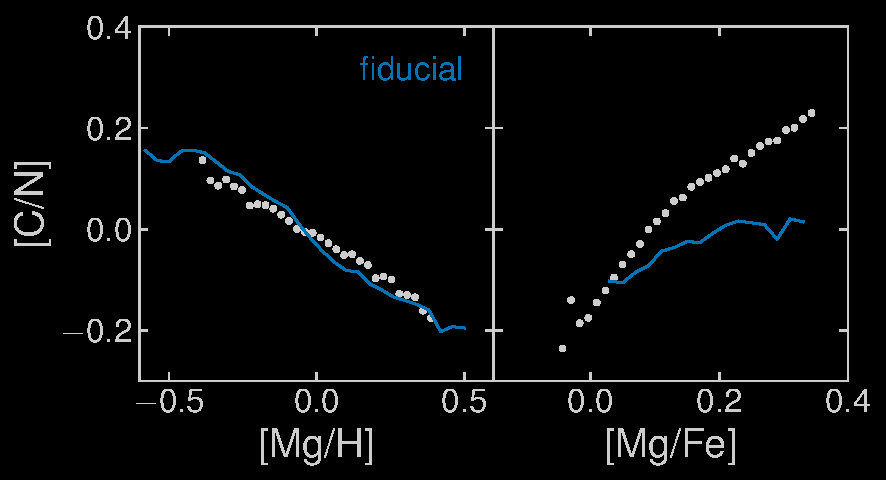
\includegraphics{c_n.pdf}
    \caption{Similar to as Figure \ref{fig:agb_sims}, except I only show the fiducial model and I plot the [C/N] abundance ratio on the y-axis.
    }
\end{figure}

\begin{figure*}
\centering
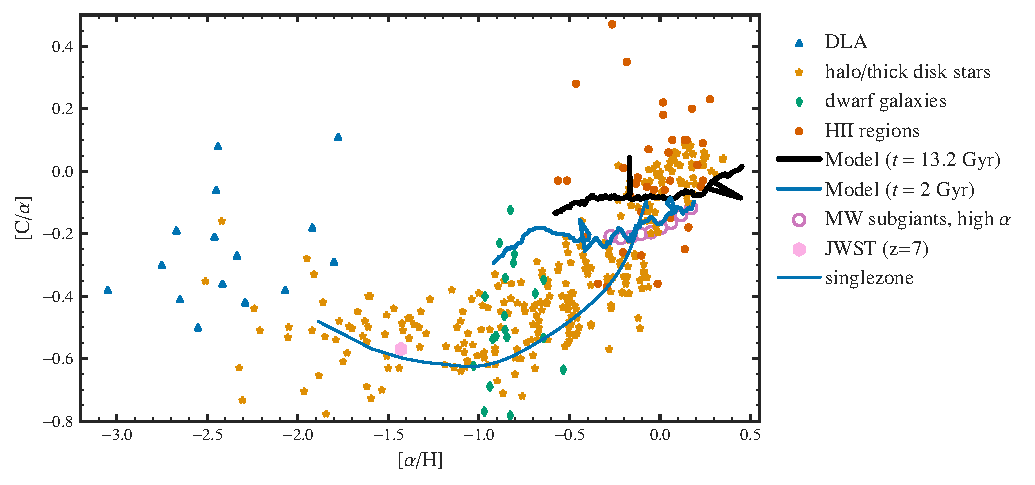
\includegraphics[]{summary.pdf}
\caption[Gas phase abundances]{Gas-phase C abundances. We plot our model at $t=2$Gyr and present day as thick solid lines. Points represent measurments in 
    HII regions    \citep[pink circles;][]{skillman+20, esteban+02, esteban+09, esteban+14, esteban+19}
    Damped Lynman-$\alpha$ (DLA) systems \citep[blue triangles;][]{cooke+17} 
    Milky Way halo and thick disk stars \citep[green stars;][]{nissen+14, fabbian+09}. 
    dwarf galaxies \citep[red diamonds;]{berg+19},
    and Milky Way high-$\alpha$ stars (yellow points; \citealtjack)
}
\label{fig:gas_phase}
\end{figure*}


\chapter{Conclusions}

In this work, I investigate the role of C yields on the predictions of multizone GCE models. \citet{james+22} performed a similar analysis, except focusing on N. \citet{james+22} found, to match APOGEE/\citet{fiorenzo+21}'s observations, $y_{\rm N}^{\rm AGB} \sim M Z$. 

Here, I perform a similar analysis on C. I summarize the current theoretical nucleosynthetic predictions of C. Because CCSNe C yields are poorly understood, I adopt an equilibrium approximation and determine that a functional form of $\Ycc/\Yoc=1.51 + 0.54 (Z/Z_\odot)$ approximately matches trends in APOGEE subgiants. Variations of the metallicity dependence of this CCSNe yield affect trends in \caah but do not affect trends in \caafe when taking a slice in [Mg/H]. As all theoretical AGB C yields decrease with increasing metallicity, increasing the AGB fraction causes the \caah trend to flatten. However, the \caafe trend is sensitive to the AGB fraction. 
I estimate that $f_{\rm AGB} = 0.2$ using the C11 yield model. This requires about 3x more AGB C production than most nucleosynthetic models predict.

Evolutionary history

Finally, I compare my model against gas phase and metal-poor stellar measurments. While my model was built on data near solar metallicity, by including heightened C production from population III stars, I can create a self consistant picture of C evolution.

Observations of C in metal poor stars, extragalactic (call out any

Implications in Stellar evolution

These C yield constraints provide a test for stellar evolution models. C yields are sensitive to mass loss treatment, explodability, nuclear cross sections, convection, and stellar structure. 

Future surveys such as the Milky Way Mapper will enable further refinement of galactic trends, placing yet more stringent constrants on stellar evolution models.
MWM and value of this work

existing surveys in e.g. APOGEE/DESI?)
Abundance ratios (e.g.C12/C13) as additional constraints



%%%%%%%%%%%%%%%%%%%% REFERENCES %%%%%%%%%%%%%%%%%%

% The best way to enter references is to use BibTeX:

\newpage
\bibliographystyle{aasjournal}
\addcontentsline{toc}{chapter}{Bibliography}
\bibliography{main} % if your bibtex file is called example.bib


% Alternatively you could enter them by hand, like this:
% This method is tedious and prone to error if you have lots of references
%\begin{thebibliography}{99}
%\bibitem[\protect\citeauthoryear{Author}{2012}]{Author2012}
%Author A.~N., 2013, Journal of Improbable Astronomy, 1, 1
%\bibitem[\protect\citeauthoryear{Others}{2013}]{Others2013}
%Others S., 2012, Journal of Interesting Stuff, 17, 198
%\end{thebibliography}

%%%%%%%%%%%%%%%%%%%%%%%%%%%%%%%%%%%%%%%%%%%%%%%%%%

%%%%%%%%%%%%%%%%% APPENDICES %%%%%%%%%%%%%%%%%%%%%

\appendix
\chapter*{Appendix}
\addcontentsline{toc}{chapter}{Appendix}
\renewcommand{\thesection}{A.\arabic{section}}
\renewcommand\thefigure{A\arabic{figure}}    
\renewcommand\theequation{A\arabic{equation}}    
\setcounter{figure}{0}
\setcounter{equation}{0}



\section{The APOGEE Subgiant Sample}\label{sec:jack}

I use the criteria outlined in \citetjack~to create a sample of subgiants from APOGEE DR17 \cite{apogee17} as our primary observational constraint. Subgiants are reflective of birth abundances for CNO \citep{souto19}. with chemical abundance determinations from ASPCAP \citep{aspcap}. SDSS 17 \cite{sdss17}.
\citetjack~selects a region of stars in $\log g$-$T_\text{eff}$ space described by the following polyhedron
\begin{equation}
    \begin{cases} \label{eq:subgiant_selection}
        \log \text{g} \geq 3.5 \\
        \log \text{g} \leq 0.004T_{\rm eff} - 15.7 \\
        \log \text{g} \leq 0.000706T_{\rm eff} + 0.36 \\
        \log \text{g} \leq -0.0015T_{\rm eff} + 12.05 \\
        \log \text{g} \geq 0.0012T_{\rm eff} - 2.8 \\
    \end{cases}
\end{equation}

\begin{figure}
    \centering
    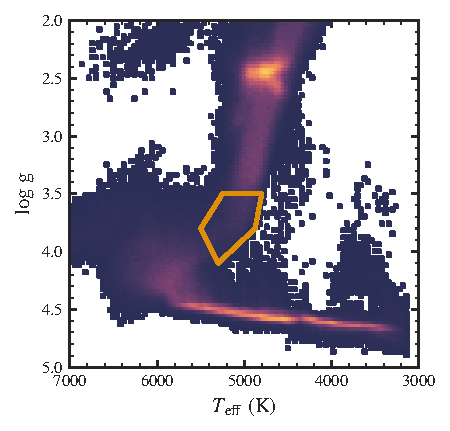
\includegraphics{logg_jack.pdf}
    \caption[Subgiant selection]{
        A Kiel diagram of APOGEE stars. Following \citetjack, we select subgiants in the orange polygon (see Equation \ref{eq:subgiant_selection}). These stars have not yet experienced first dredge-up, so their photospheric C and N abundances should reflect their birth mixture.
    }
\end{figure}

This cut isolates a clean sample of subgiants. As first dredge up, which affects C and N abundances, only occurs during the ascent onto the red giant branch, subgiant stars are unaffected by this enrichment. 

Additionally, I exclued stars in APOGEE marked by the following flags.
\begin{itemize}
\item \verb|APOGEE_MIRCLUSTER_STAR|
\item \verb|APOGEE_EMISSION_STAR|
\item \verb|APOGEE_EMBEDDEDCLUSTER_STAR|
\item \verb|young cluster (IN-SYNC)|
\item \verb|APOGEE2_W345|
\item \verb|EB planet|
\end{itemize}

A second approach in determining birth abundances in stars is to correct the surface abundance effects of FDU, as in \cite{fiorenzo+21}. I note that there is a slight difference in the yields found through \cite{fiorenzo+21} and \citetjack. As o

\begin{equation}\label{eq:high_alpha}
\begin{cases}
\text{[Mg/Fe]} >0.12-0.13\text{[Fe/H]}, & \text{[Fe/H]}<0\\
\text{[Mg/Fe]} >0.12, & \text{[Fe/H]}>0\\
\end{cases}
\end{equation}



I choose to use \citetjack's sample as this does not rely on additional layers of modeling, providing a more direct constraint to our model and limiting our systematic uncertainties.

\newpage
\section{Additional Considerations of Yields}\label{sec:alt_agb}


While I focus the main discussion of the paper on the C11 model, other AGB models can have notable effects on abundance trends at ***

Because the predictions of the AGB yield models I consider are dwarfed by the
required CCSNe C production to match observations (see Fig. ***), I briefly explore here the effects of variations in AGB models affect abundance trend predictions when these models are amplified to match observational [C/MG]-[Mg/Fe] trends. 

While most models are well represented by our AGB-fraction formalism, V13 presents a challenge as the predicted solar yield is much lower than the lower metallicity predictions, requiring the solar value to be a certain fraction forces us to amplify the yields by an unreasonable about (of order 10-30times) to reach the same $f_{\rm AGB}$ as other models. Thus, I instead calculate $f_{\rm AGB}$ at a metallicity of ... for this model. 

V13 is also interesting as at high metallicity, the yields quickly become strongly negative. This causes a reversal of the [C/Mg]-[Mg/Fe] trend at high [Mg/H] slices (figure ...). As our set of observations do not appear to reverse, this indicates that C yields likely stay positive even at slightly super-solar, so models like V13 are a poor match to observations. 
Plot of age metallicity relationship?


\begin{figure}[htp]
    \centering
    \includegraphics{agb2.pdf}

    \caption[Alternate AGB models]{Same as Figure \ref{fig:agb_sims} except where $f_{\rm agb}=0.2$. When yields are amplified, chaos ensues.}
\end{figure}


\begin{figure}
    \centering
    \includegraphics{y_mg.pdf}
    \caption[Magnesium CCSNe yields]{Same as the top panel of Figure \ref{fig:y_cc}, but for Mg. Our Mg yield choice is shown as a dashed line at the top
    }
\end{figure}

\begin{figure}
    \centering
    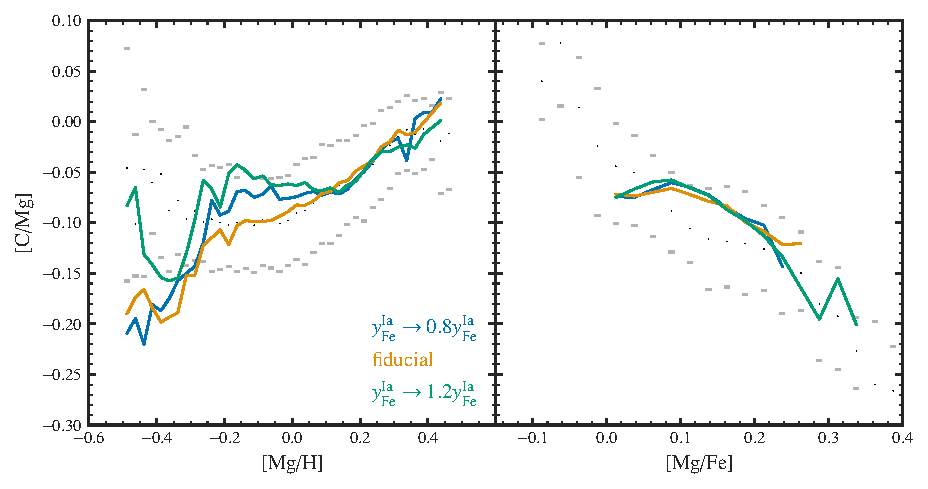
\includegraphics{fe_ia.pdf}
    \caption[Adjusting type Ia iron]{Similar to Figure \ref{fig:agb_sims} except with variations of the SNeIa iron fraction}
\end{figure}




\newpage

\section{Software}

Software which has contributed to this work:

\begin{itemize}
    \item \citet{OhioSupercomputerCenter1987}
    \item \VICE~\citep{JW20, james+21}
    \item \texttt{matplotlib} \citep{matplotlib}
    \item \texttt{scipy} \citep{scipy}
    \item \texttt{IPython} \citep{ipy}
    \item \texttt{pandas} \citep{pandas}
    \item \texttt{numpy} \citep{numpy}
    \item \texttt{astropy} \citep{astropy:2013, astropy:2018, astropy:2022}
    \item \texttt{seaborn}
\end{itemize}


\label{lastpage}
\end{document}




